\documentclass[11pt]{article}
\usepackage{url,amsmath,setspace,amssymb,amsthm,fullpage}
\usepackage{tikz}
\usetikzlibrary{arrows}
\usepackage{algorithm}
\usepackage[noend]{algpseudocode}

\makeatletter
\def\BState{\State\hskip-\ALG@thistlm}
\makeatother

% Scribe template modified from original created by UC Berkeley's EECS department

\newcommand{\heading}[5]{
   \renewcommand{\thepage}{#1-\arabic{page}}
   \noindent
   \begin{center}
   \framebox[\textwidth]{
     \begin{minipage}{0.9\textwidth} \onehalfspacing
       {\bf STATS 710 -- Seq. Dec. Making with mHealth Applications} \hfill #2

       {\centering \Large #5

       }\medskip

       {\it #3 \hfill #4}
     \end{minipage}
   }
   \end{center}
}
\newcommand{\scribe}[4]{\heading{#1}{#2}{Instructors:
Susan Murphy and Ambuj Tewari}{Scribe: #4}{Lecture #1: #3}}

\newtheorem{lemma}{Lemma}
\newtheorem{theorem}[lemma]{Theorem}
\newtheorem{proposition}[lemma]{Proposition}

\newtheorem{definition}{Definition}

\newcommand\reals{\mathbb{R}} % real numbers
\newcommand\E[1]{\mathbb{E}\left[ #1 \right]} %expectation

\bibliographystyle{alpha}

\begin{document}
\scribe{21}{Nov 29, 2016}{Partial feedback and combinatorial action space}{Yutong Wang}
\section{Motivation}
Suppose that the learner commutes from home to work along routes shown by the graph below. 

\begin{figure}[h]
    \centering
    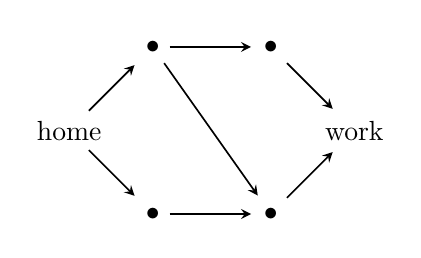
\begin{tikzpicture}[
            > = stealth, % arrow head style
            shorten > = 1pt, % don't touch arrow head to node
            auto,
            node distance = 1.5cm, % distance between nodes
            semithick % line style
        ]

        \tikzstyle{every state}=[
            draw = black,
            thick,
            fill = white,
            minimum size = 4mm
        ]

        \node (s) {home};
        \node (v1) [above right of=s] {$\bullet$};
        \node (v2) [below right of=s] {$\bullet$};
        \node (v3) [right of=v1] {$\bullet$};
        \node (v4) [right of=v2] {$\bullet$};
        \node (t) [below right of=v3] {work};

        \path[->] (s) edge node {} (v1);
        \path[->] (s) edge node {} (v2);
        \path[->] (v1) edge node {} (v3);
        \path[->] (v2) edge node {} (v4);
        \path[->] (v3) edge node {} (t);
        \path[->] (v4) edge node {} (t);
        \path[->] (v1) edge node {} (v4);
    \end{tikzpicture}    
\end{figure}

Each arrow represents a subroute and has some amount of congestion. The learner's goal is to pick a path from home to work that has low congestion. Let $\mathcal{A}$ denote all path from home to work. We can think of this as a bandit problem where the arms are the paths $\mathcal{A}$. In this example, the rewards could be highly correlated between the arms. Thus, we may get much better regret bounds if we consider this correlation structure. Furthermore, it may be the case that the learner gets only partial feedback, e.g.\ only the congestion on a subroute of the path is revealed. Finally, combinatorial action spaces such as the above tend to be large, which means applying bandit algorithms out of the box could be impractical. For all the preceding reasons, the partial feedback and combinatorial action space setting deserves some special attention.

\section{Online ranking with top-1 feedback}
We consider the problem of online ranking of $K$ items by relevance where we only receive feedback for the top ranked item. For a real world scenario, suppose that we own a restaurant that serves $K$ dishes and we would like the menu to display the most relevant dishes on top. The menu is digital and can rearrange itself in real time. In order to not annoy the customers, we only collect feedback for the top menu item. The goal to learn a ranking that ranks the relevant dishes as high as possible.

Below, let $K$ be a positive integer. Following group theory notations, let $\mathcal{A} = S_K$ be the set of permutations on $\{1,\dots, K\}$. In other words, an element $\sigma$ of $S_K$ is a bijection from $\{1,\dots, K\}$ to itself. For each $i = 1,\dots, K$, we think of $\sigma(i)$ as the ranking of the $i$-th item (lower is better). Let $T$ denote the time horizon. The protocol is as follows. 

For $t = 1,\dots, T$:
\begin{enumerate}
    \item Learner takes action $\sigma_t \in S_K$
    \item Nature selects $\rho_t \in \{0,1\}^K$, where $\rho_t(i) =1$ if and only if the $i$-th item is relevant.
    \item Learner observes $\rho_t(\sigma_t^{-1}(1))$, i.e.\ only the relevance of the top ranked item is revealed.
    \item Learner suffers loss $\rho_t^T \sigma_t := \sum_{i=1}^K \rho_t(i) \sigma_t(i) = \sum_{i: \rho_t(i) = 1} \sigma_t(i)$
\end{enumerate}


The expected regret is defined as 
\begin{equation}\label{expected regret}\mathcal{R}(\mathcal{L},T) \equiv \mathbb{E}\left[ \sum_{t=1}^T \rho_t^T \sigma_t\right]  - \min_{\sigma \in S_K} \sum_{t=1}^T \rho_t^T \sigma\end{equation}
Using algorithm \ref{main algorithm} below as the learning algorithm $\mathcal{L}$, we can achieve \begin{equation}\label{expected regret bound}\mathcal{R}(\mathcal{L},T) \sim O(\mathrm{poly}(K)T^{2/3})
\end{equation}which is in fact optimal and strictly harder than a bandit problem. Note that in the bandit feedback setting, i.e.\ we have knowledge of $\rho_t^T \sigma_T$ in step 3, then $\mathcal{R}(\mathrm{EXP}(3), T) \sim O(\exp(K)\sqrt{T})$.
\subsection{A learning algorithm}
We split the $T$ rounds into $L$ blocks, with $L$ to be determined later. Write $B_i = \left((i-1)\frac{T}{L}+1, \dots, i\frac{T}{L}\right)$ to denote the $i$-th block. For each $i$, sample $K$ indices without replacement from $B_i$ and denote these indices by $I^{(i)}_1,\dots, I^{(i)}_K$. During the $I^{(i)}_j$-th round, we rank the $j$-th item on top and rank the rest arbitrarily, i.e.\ choose $\rho_{I^{(i)}_j} \in S_K$ such that $\rho_{I^{(i)}_j}(j) = 1$. Let $\hat \rho_i = \left(\rho_{I^{(i)}_1}(1),\dots, \rho_{I^{(i)}_K}(K)\right)$.
\begin{lemma}
$\hat \rho_i$ is an unbiased estimator for $\sum_{t \in B_i} \rho_t/|B_i|$.
\end{lemma}
Here is the overall learning algorithm from \cite{chaudhuri2015online} 
\begin{algorithm}
\caption{}\label{main algorithm}
\begin{algorithmic}[1]
\State Given parameters $T, L, \epsilon, B_i$ as above
\State Initialize $\hat s_0 = \vec{0}$ as the zero vector
\For{$i=1,\dots, L$}
\State $\hat{s}_{i-1} = \hat s_{i-2} + \hat \rho_{i-1}$
\For{$t \in B_i$}
\State Sample $I^{(i)}_1,\dots, I^{(i)}_K$ from $B_i$ without replacement.
 \If{$t = I^{(i)}_j$ for some $j=1,\dots, K$} \State {Output any $\sigma_t$ such that $\sigma_t(j) =1$} 
 \State {Receive $\rho_{I^{(i)}_j}$}
 \Else 
 \State{Draw $Z_t \in [0,1/\epsilon]^K$ so that the coordinates are independently and uniformly sampled from $[0,1/\epsilon]$}
 \State \label{FTPL}{Output $\sigma_t = \argmin_{\sigma \in S_K} \sigma^T(\hat s_{i-1} + Z_t)$}
 \EndIf
\EndFor
\EndFor
\end{algorithmic}
\end{algorithm}

Line \ref{FTPL} is known as ``follow the perturbed leader" (FTPL) \cite{kalai2005efficient} where $Z_t$ is the perturbation. In the stochastic setting, it is okay to leave out $Z_t$, which is known as simply ``follow the leader" (FTL). However, in the adversarial setting, the adversary may exploit the determinism in FTL and result expected regret linear in $T$.
\subsection{Full information version of the ranking problem}
From the perspective of the outer for loop of algorithm \ref{main algorithm}, the protocol is as follows. For $t = 1,\dots, L$:
\begin{enumerate}
    \item Learner takes action $\sigma_t \in S_K$
    \item Nature reveals the entire vector $\rho_t \in \{0,1\}^K$
    \item Learner suffers loss $\rho_t^T \sigma_t := \sum_{i=1}^K \rho_t(i) \sigma_t(i) = \sum_{i: \rho_t(i) = 1} \sigma_t(i)$
\end{enumerate}

The regret is still defined as in (\ref{expected regret}).
\begin{theorem}[\cite{kalai2005efficient}]
Consider FTPL $\sigma_\tau = \argmin_{\sigma \in S_K} \sigma^T(\sum_{s=1}^{\tau-1} \rho_s + Z_t)$ as a learning algorithm for the protocol above. If $\|\sigma_\tau\|_1 \le B_\sigma$, $|\sigma_\tau^T \rho_\tau| \le B_{\text{loss}}$ and $\|\rho_\tau\|_1 \le B_{\rho}$ then for $\epsilon = \sqrt{\frac{B_\sigma}{B_{\text{loss}}B_\rho L}}$, the expected regret of FTPL is $2 \sqrt{B_\sigma B_{\text{loss}} B_\rho L}$.
\end{theorem}
Note that to use the theorem for the outer loop in algorithm \ref{main algorithm}, we can let $B_\sigma = B_{\text{loss}} = K^2$ and $B_\rho = K$ in the theorem. Next time, we will apply the theorem to our setting to prove (\ref{expected regret bound}).
\bibliography{stats710}

\end{document}


